

%\begin{sciabstract}
%In recent decades, liquid xenon time projection chambers (TPCs) have placed the most stringent limits on the cross-section of particulate dark matter in the form of weakly interacting massive particles (WIMPs). One of the largest factors in the success of these detectors is the purity of the xenon used as the WIMP target material. It is therefore important for the outgassing of impurities from plastic internals of these detectors to be quantified and if necessary mitigated. 

%The LUX and LZ dark matter detectors use polyethylene (HDPE), Teflon (PTFE), and Viton in various parts that contact the target xenon. Measured values of the constants of permeation for suspect impurities such as krypton, argon, nitrogen, and methane can be used to predict impurity loads and optimize mitigation measures
%\end{sciabstract}


\chapter{Cosmology Overview}
\section{Standard Model of Cosmology}
The standard model (SM) ties together observations and theories of particle physics into a coherent and predictive picture that is well verified by experiment. In the same way, the standard model of cosmology ($\Lambda$-CDM) combines the observations of astronomers and cosmologists in the context of general relativity. Although the standard model paints a comprehensive picture of particles that have been observed, it accounts for only 4.9\%\cite{planck2015} of the mass-energy content of the $\Lambda$-CDM model. 

The $\Lambda$-CDM model is built on the foundation of the Robertson-Walker metric:
\begin{equation} \label{eq:rwmetric}
ds^2 = -c^2dt^2+a(t)^2 \left[ dr^2 +S_{\kappa}(r)d\Omega \right]
\end{equation}
\begin{equation}\label{eq:rwcurvature}
S_{\kappa}(r)=
\begin{cases}
R_0sinh(r/R_0) & \text{for } \kappa = 1 \\
r                        & \text{for } \kappa = 0 \\
R_0sin(r/R_0)   & \text{for } \kappa = -1
\end{cases}
\end{equation}
This metric assumes an isotropic and homogenous universe, but allows for both time dependent expansion and uniform curvature. The unitless ``scale factor'', $a(t)$, describes the expansion and contraction of the spatial part of the metric. The curvature of space is characterized by a radius of curvature $R_0$ and the parameter $\kappa$, which is 0 if the universe is flat and otherwise indicates the sign of the curvature.

The time-dependence in the scale factor can now be described to first and second order. The Friedmann equation is a solution to Einstein's field equations that relates the rate of change in the scale factor to the energy density of the universe, $\varepsilon$:
\begin{equation}\label{eq:friedmann}
H^2 \equiv \left( \frac{\dot{a}}{a} \right)^2 = \frac{8\pi G}{3c^2}\varepsilon - \frac{\kappa c^2}{R_{0}^{2}a^2},
\end{equation}
where $G$ is the gravitational constant. Equation \ref{eq:friedmann} also introduces the Hubble constant, $H$, which describes the expansion rate of the scale factor. The second order equation is obtained through an application of the first law of thermodynamics for an adiabatically expanding universe. This gives the fluid equation, which connects the change in energy density to pressure:
\begin{equation}\label{eq:fluid}
\dot{\varepsilon} + 3 \frac{\dot{a}}{a}(\varepsilon +P)=0 
\end{equation}
By combining equations \ref{eq:friedmann} and \ref{eq:fluid}, the acceleration equation is found:
\begin{equation}\label{eq:accel}
\frac{\ddot{a}}{a} =  -\frac{4\pi G}{3c^2}(\varepsilon+3P).
\end{equation}

In an empty universe where $\varepsilon$ is zero, the time evolution of the scale factor is trivial. The curvature can be either flat or negative, but a positive curvature would lead to a non-physical result in equation \ref{eq:friedmann}. In a flat, empty universe the scale factor would be static, and in a negatively curved universe, the scale factor would increase at a constant rate for all time. To describe the time-evolution of the scale factor in a universe where $\varepsilon \neq 0$, there is one further puzzle piece required. A universe can contain multiple component energy densities which will each contribute a unique pressure. The relation between the total energy density and pressure is given by the equation of state:
\begin{equation}
P= \sum_w w\varepsilon_w,
\end{equation}
where $w$ is a parameter specific to each component.

The total energy density is equal to the sum of the component densities, $\varepsilon_{w}$. These are often normalized to the critical density, $\varepsilon_{c} = \frac{3c^2}{8\pi G}H(t)^2$ and expressed as density parameters, $\Omega_{w}=\varepsilon_{w}/\varepsilon_{c}$. The components of interest in this universe are radiation (which includes relativistic matter), non-relativistic matter, and a contribution from the cosmological constant, $\Lambda$ (also referred to as dark energy), for which $w = 1/3, 0, -1$ respectively. Radiation and matter both act to slow down the expansion rate of the universe, while $\Lambda$ acts to accelerate it. This can be seen more clearly by examining the scale factor in the case of a universe with a single component energy density. The time dependences of the scale factor for single component universes are shown in Table \ref{table:energy components}.

\begin{table}[h!]
\begin{center}
  \begin{tabular}{ c | c  }
    Single Energy Component & $a(t)$ \\ \hline
    \hline
    Negative Curvature & $t/t_{0}$  \\ \hline
    Matter & $(\frac{t}{t_{0}})^{2/3}$  \\ \hline
    Radiation & $(\frac{t}{t_{0}})^{1/2}$  \\ \hline
    $\Lambda$ & $e^{H_{0}(t-t_{0})}$ \\
  \end{tabular}
\end{center}
\caption{Here is shown the time dependence of the scale factor, $a$, in various single energy component universes.}\label{table:energy components}
\end{table}

Matter, radiation, and $\Lambda$ themselves have different dependences on $a(t)$. Matter density is related to the number density of particles, so as $a(t)$ increases, $\varepsilon_{matter}$ will decrease like $1/a(t)^{3}$. In addition to it's dependence upon number density, $\varepsilon_{radiation}$ also has a dependence upon the frequency of the radiation. Since an increasing $a(t)$ stretches the radiation's wavelength, thereby decreasing its frequency, $\varepsilon_{radiation}$ will gain an additional factor of $1/a(t)$ in its time dependence, so $\varepsilon_{radiation}$ will decrease proportional to $1/a(t)^{4}$\cite{ryden}.

The most widely accepted and best supported model for the current universe has no curvature, is old enough that the radiation component has become negligible, and contains a comparable density of matter and $\Lambda$. This model is referred to as the $\Lambda$-CDM model. 

\section{The Cosmic Microwave Background}
The various parameters for the $\Lambda$-CDM model are best constrained by measurements of the cosmic microwave background by the Planck experiment, which constrains $\Omega_{matter}$ to $0.3089 \pm 0.0062$ and $\Omega_{\Lambda}$ to $0.6911 \pm 0.0062$\cite{planck2015}. The Planck experiment, along with its predecessors, aimed to create a detailed map of the cosmic microwave background. This background is a snapshot of the universe from only 350,000 years after the big bang.\cite{ryden} Before that time, the universe was hot enough that electrons could not bind to protons to form atoms, and the scattering rate of photons off of this plasma was high enough for them to thermalize into a blackbody spectrum. Once the scattering rate of high energy photons dropped below the expansion rate of the universe, electrons and protons began forming atoms, which in turn lowered the scattering rate even more. This caused the blackbody photons to rapidly become decoupled from the matter, thus preserving their blackbody spectrum. These photons are what today form the cosmic microwave background (CMB).

Due to random fluctuations, there were anisotropies in the primordial plasma, which tended to fall toward areas with higher densities. This caused the over-densities to become amplified until eventually the increased radiation pressure would overtake the force of gravity, causing the plasma to rebound and expand until the now falling pressure was overtaken the gravitational pull of the over-density. This process led to a ``ringing'' in the primordial plasma, which is referred to as baryon acoustic oscillations (BAO). BAO began at the end of the inflationary period and ended after the epoch of recombination, when photons decoupled from protons and electrons. 

BAO can be seen today as ripples in the CMB. These ripples can be most clearly seen in the angular correlation power spectrum of the CMB shown in Figure \ref{fig:powerspectrum}. The highest peak at $l \approx 200$, corresponds to about $1^{\circ}$, the angular scale at which the plasma had time to fall into its first compression before photon-decoupling. The second peak corresponds to the scale at which plasma had time to compress and rebound to its first rarefaction. The higher-$l$ peaks show this processes repeating itself, with odd numbered peaks corresponding to compressions and even numbered peaks corresponding to rarefactions. 

\begin{figure}[h!]
\centering
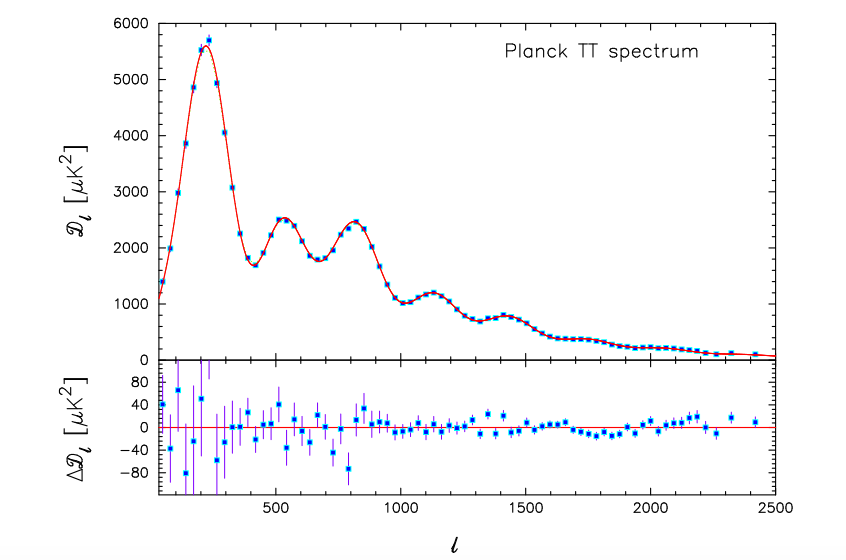
\includegraphics[width=150mm]{Figures/PLANCK_PS_TT}
\caption{Angular correlation power spectrum of the CMB as measured by the Planck experiment. The red line shows the best fit spectrum assuming the $\Lambda$-CDM model. \cite{planck2015}}
\label{fig:powerspectrum} 
\end{figure}


\section{Dark Matter}
There is one piece of the $\Lambda$-CDM puzzle that is conspicuous in its absence from the description so far. Cold Dark Matter (``CDM'' in ``$\Lambda$-CDM'') is one of the key elements of the model. Without a driving force external to the photon-baryon plasma, the baryon acoustic oscillations would decay exponentially. The prominence of the third peak relative to the first and second points to the need for an additional form of matter. This matter would be out of equilibrium with the plasma, and so would collapse into the primordial over-densities, but not experience a restorative pressure. As the baryons oscillate, this ``dark matter'' would continue to accumulate, strengthening the gravitational well. This matter would necessarily couple strongly to neither itself, nor the photons or baryons in the plasma. 


\subsection{Galaxy Clusters}
The evidence for dark matter from the CMB is relatively recent. Astronomers have been chasing the missing matter problem for almost a century. The first conclusive evidence for what is now know as dark matter came from Fritz Zwicky's observations of the velocity distribution of galaxies in the Coma Cluster in 1933\cite{zwicky}, although calculations by Jan Oort of stellar velocities in the Sombrero galaxy hinted that something was amiss a year earlier in 1932\cite{oort}. Assuming that the galactic velocities in the Coma cluster are in a stationary state, the virial theorem can be applied:
\begin{equation}\label{eq:virial1}
\bar{V}=-2\bar{K},
\end{equation}
where $\bar{V}$ is the average total potential energy of the system, and $\bar{K}$ is the average total kinetic energy of the system. Assuming a spherically symmetric system governed by Newtonian gravity, Zwicky then made the following approximations for his calculations:

\begin{equation}\label{eq:potential}
V \approx \frac{-3GM}{5R}
\end{equation}
\begin{equation}\label{eq:kinetic}
K \approx \frac{1}{2}M \bar{\bar{v}}^{2},
\end{equation}
where $M$ is the total mass of the cluster, and $\bar{\bar{v}}$ is the velocity of galaxies in the cluster, averaged over time and mass. Using observations of the doppler shift of the light coming from galaxies within the cluster, Zwicky was able to measure the component of the velocities along the line of sight. He then made the assumption that the velocities are isotropic in order to extrapolate to the overall distribution, $\bar{\bar{v}}=\bar{v}_{LS}$.

Using this method, Zwicky placed a conservative limit of $M > 4.5 \cdot 10^{13}_{\odot}$ on the mass of the Coma cluster. Comparing this result to the amount of light coming from the cluster, he found that the mass-to-light ratio was more than 100 times larger than typical values for local stellar systems. This was the first indication that a large percentage of matter in the universe is not luminous\cite{zwicky}.

\subsection{Galactic Rotation Curves}
Continuing from the early measurements of the spiral galaxies by Jan Oort, it was further observed that the other galaxy types also display strong evidence of containing dark matter\cite{persic}.  A spiral galaxy is well approximated by a flat disk. This makes it possible to measure its galactic rotation curve, or the orbital velocity as a function of radius. Measurements of galactic rotation curves provide some of the most clear and compelling evidence for both the existence and behavior of dark matter on galactic scales.

Measurement's of the luminosity of galaxies show that the density of visible matter tends to decrease exponentially with radius from the galactic center:
\begin{equation}\label{eq:luminosity}
I(R)=I_{0}e^{-R/R_{s}},
\end{equation}
where R is the radius from the galactic center, and $R_{S}$ is the a length scale specific to each galaxy. For the Milky Way $R_{S}$ is about 4 kpc\cite{ryden}. This exponential drop would lead rotation curves proportional to $1/\sqrt{R}$. In contradiction to this, spectroscopic measurements of stars near the galactic center and the H$\alpha$ line outside of the optical radius, show that the rotation curves of spiral galaxies tend to become flat at large radii\cite{rubin, persic}. Beginning with Vera Rubin in 1980 \cite{rubin} and continuing with Massimo Persic and Paolo Salucci \cite{persic} among others, researchers went on to characterize the rotational velocities of spiral galaxies by a ``universal rotation curve'' (URC). 

\begin{figure}[h!]
\centering
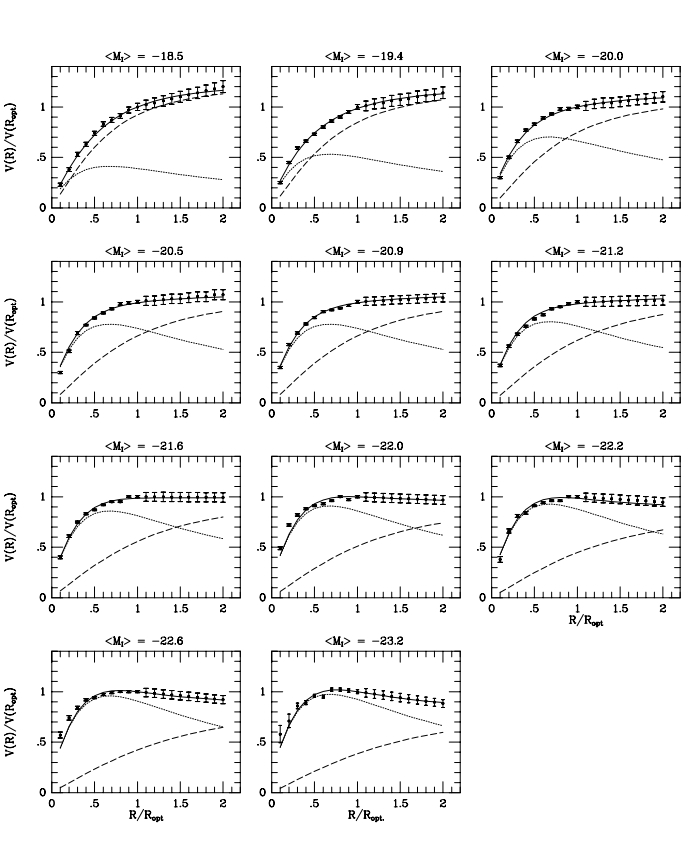
\includegraphics[width=150mm]{Figures/persic_salucci_urc}
\caption{URC (solid lines) fit to average rotation curves surveyed spiral galaxies. The subfigures show bins in luminosity each of which contain about 50 individual rotation curves. Also shown are the contributions from the luminous disk (dotted line) and dark halo (dashed line)\cite{persic}.}
\end{figure}



The URC has two components, one from the luminous, exponentially decreasing disk and the other from a ``dark halo'' which surrounds the galaxy. This dark halo can be thought of as a gas which permeates and surrounds the disk. As a function of $R/R_{opt}$, the mass and velocity contributions from this component are:
\begin{equation}\label{eq:halo_velocity}
V_{d}^{2}=V^{2}(R_{opt})(1-\beta)(1+a^{2}) \frac{x^{2}}{x^{2}+a^{2}},
\end{equation}
\begin{equation}\label{eq:halo_velocity}
M_{h}(x)=G^{-1}V^{2}(1)R_{opt}(1-\beta)(1+a^{2}) \frac{x^{3}}{x^{2}+a^{2}}.
\end{equation}
Both $\beta$, the fraction of disk mass inside of the optical radius, and a, the radius of the halo core are completely determined by the luminosity in this model. The URC fits the observed data very well (on average fitting errors are within 1\%).


More recently, models based on n-body simulations of cold dark matter have become more popular. The most well known of these is the Navarro-Frenk-White (NFW) model. These models produce good fits to high-luminosity galaxies such as the Milky Way, but tend to produce cusps at the galactic center and have trouble replicating the flat cores observed in dwarf galaxies. It is possible that this tension could be resolved by gravitational fluctuations or by substructure within the halo at the center of these dwarf galaxies, but the ``Cusp-Core'' problem remains an active area of study\cite{weber, navarro}.




\subsection{Modified Neutonian Dynamics}

The agreement between observation of galactic rotation curves and cluster dynamics is quite remarkable, however there is an alternate hypothesis to dark matter that fits the data equally well in many of these cases. Modified Newtonian Dynamics (MOND) postulates that the force of gravity as described by Newton and Einstein is incomplete. In 1983, Milgrom showed that an interpolating function, $\mu$, could be added to Newton's second law to describe the dynamics of galaxies and clusters without the need for dark matter.
\begin{equation}\label{eq:interp_func}
m_{g}\mu(a/a_{0})\vec{a}=\vec{F}
\end{equation}
This interpolating function would be $\approx 1$ at large accelerations, $a\gg a_{0}$, reproducing the classical equation of motion, but would approach $\mu{x}=x$ when $a\ll a_{0}$, where $a_{0}=2 \times 10^{-8} cm\cdot s^{-2}$ is a fundamental constant\cite{milgrom, bekenstein}. 

Following their initial paper in 1983, M. Milgrom and J. Bekenstein reformulated MOND as a classical, lagrangian based field theory, known as AQUAL. In 2004 Bekenstein again reformulated MOND in the context of general relativity. This new tensor-vector-scalar covariant theory is referred to as TeVeS\cite{bekenstein}. Both of these theories can produce good fits to galactic rotation data in many cases, but among other problems, neither can fully describe cluster dynamics without the addition of some dark matter\cite{bekenstein, chaichiana}.

\subsection{Gravitational Lensing}
One of the single most compelling pieces of evidence for dark matter, especially in relation to MOND theories, comes from gravitational lensing data of galactic cluster 1E 0657-56, more commonly known as the bullet cluster. This cluster consists of two subclusters that recently collided and passed through each other. One of these subclusters displays a distinct bow shock that enabled researchers to make a precise measurement of its Mach number, thereby also measuring its velocity. The measured Mach number, $3.2_{-0.6}^{+0.8}$ corresponds to a velocity of $4500_{-800}^{+1100}km/s$\cite{markevitch}. 

During the collision, the gas from the two subclusters would be expected to experience much stronger drag than the stellar matter. This expectation was confirmed by x-ray imaging data from Chandra, which showed that the gas was lagging behind the stars. Further comparison to a mass mapping using gravitational lensing reveals additional matter populations centered near the stellar matter, which are taken to be the dark matter halos of the two subclusters. Fitting a King mass profile ($\rho=\rho_{0}(1+r^{2}/r_{c}^{2})^{-3/2}$) to the lensing data, Markevitch et. al. calculated the density of the dark matter, and limited the self interaction cross section to $\sigma/m < 1 cm^{2} g^{-1}$\cite{markevitch}.

\begin{figure}[h!]
\centering
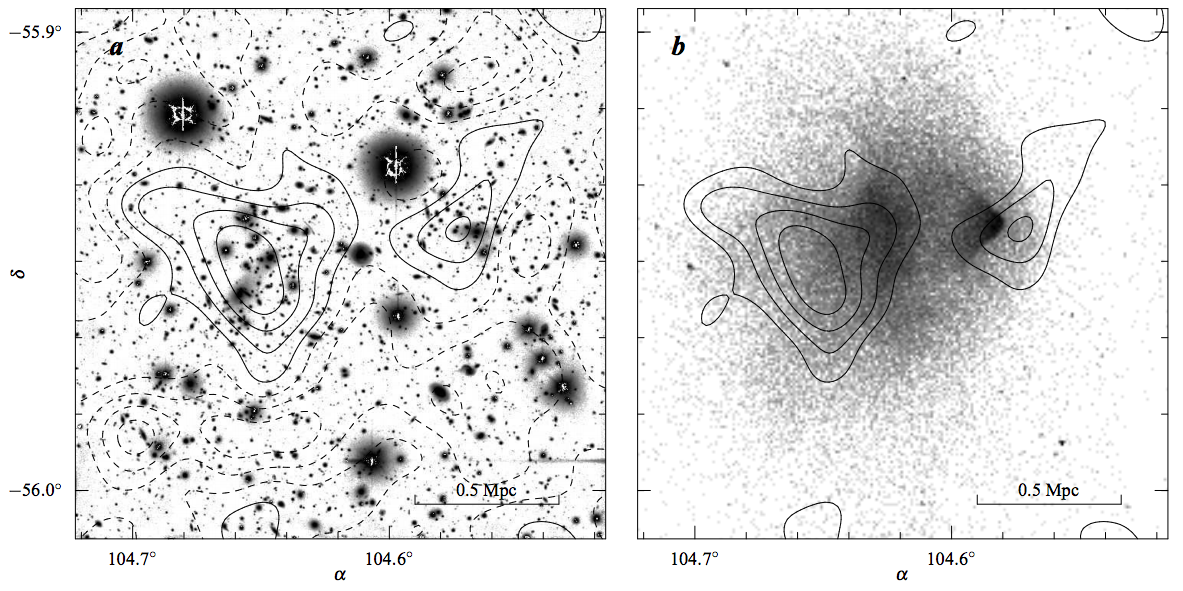
\includegraphics[width=150mm]{Figures/bullet}
\caption{Comparison of the location of dark matter, stellar matter, and x-ray gas in the bullet cluster. The mass density from lensing data, indicated by the solid black lines is imposed over optical (left) and x-ray (right) maps\cite{markevitch}.}
\end{figure}

\section{Dark Matter Candidates}
\subsection{Baryonic Dark Matter}
Now that the existence of cold dark matter has been well motivated, the next step is to investigate what it might be. A reasonable starting point is to look at types of matter that are already known to exist, and ask whether they could exist in high enough abundances to explain the observations of galaxy and cluster dynamics as well as angular correlations in the CMB.  

Within the standard model, the first place to look for dark matter is baryonic matter. It is possible, for instance, that the dark halo is, at least partially, composed of large structures of baryonic material such as brown dwarfs or planets. These massive compact halo objects (MaCHO's) should be observable through gravitational lensing. As a MaCHO passes between an observer on Earth and a background star, the light from that galaxy will be temporarily distorted through gravitational lensing. The EROS-2 experiment conducted a survey of the large Magellanic clouds and found insufficient lensing events to allow MaCHO's as a primary constituent of the Milky Way's dark halo\cite{macho}.

A more general constraint on baryonic dark matter comes from measurements of big bang nucleosynthesis (BBN). BBN refers to the epoch at which the temperature of the universe dropped below the binding energy of deuterium (2.22 MeV). This happened when the universe was about 5 minutes old. During this epoch, the primordial abundances of light nuclei are set as the protons and neutrons are allowed to combine into energetically favored favored states. The ratios of these abundances are highly dependent on $\eta$, the baryon-photon ratio, so the measurement of them, combined with constraints on the photon density from CMB measurements would give a precise value for the baryon density\cite{ryden}. Current measurements of D/H place the baryon density at $\Omega_{b} h^{2} = 0.02202 \pm 0.00046$ \cite{bbn}. This result is within $1\sigma$ of the measurement from the Planck experiment, and taking the reduced Hubble constant to be $h = 0.678$, it indicates that baryons make up only 4.8\% of the energy-density of the universe\cite{planck2015}.


\subsection{Neutrinos}
The remaining candidate for standard model dark matter is the neutrino. Before the CMB decoupled, neutrinos went through a similar process which left the universe filled with neutrinos that had been in thermal equilibrium with the extremely hot and dense early universe. From the annihilation cross-section, the number density of the cosmic neutrino background (CNB) can be calculated to be 3/11 that of CMB photons\cite{ryden},
\begin{equation}
n_{\nu}=3.36 \times 10^{8} \ m^{-3}.
\end{equation}
In order for the CNB to fit the mass density requirement for dark matter, the mass of neutrinos would have to be about $4 \ eV$.\cite{ryden}  Current constraints from Planck show that the combined mass of neutrinos is $< \ 0.23 \ eV$\cite{planck2015}, so neutrinos are not heavy enough to explain the majority  of observed dark matter.


\subsection{Axions}
Currently, the two most popular CDM candidates are Axions and WIMPs. Axions are particularly interesting because they were first theorized as part of a solution to the strong CP problem, and so could simultaneously solve two unsolved problems in physics. Charge-parity (CP) is only conserved by QCD if the vacuum angle, $\theta$, is 0. However,  $\theta$ should be able to take any value, so CP is not predicted to be conserved. Experimental measurements of the neutron electric dipole moment (nEDM) show that CP is, in fact, a good symmetry of QCD. The current limit on nEDM is about $2 \times 10^{-26} \ e \cdot cm$, which in turn limits $\theta$ to $\leq \ 10^{-9}$\cite{nedm,axion_DM}. This unexpectedly small value of $\theta$ points to a tension within QCD. To relieve this tension, R. Peccei and H. Quinn proposed a new spontaneously broken global symmetry, $U_{PQ}(1)$, and showed that if the Higgs potential for at least one quark is invariant under $U_{PQ}(1)$, then $\theta$ is guaranteed to relax to 0. The pseudo-Nambu-Goldstone boson that is associated with the spontaneous breaking of $U_{PQ}(1)$ is known as the axion \cite{peccei_quinn, axion_DM}.

The axion as a candidate for CDM is compelling in that it interacts only very weakly with standard model particles. Axions are expected to be have mass, but be light enough that those produced thermally in the big bang would be too hot to fill the role of CDM. However, populations of axions can be formed non-relativistically in the early universe through vacuum realignment and topological effects in string theory. Axion dark matter created through realignment would be expected to have a mass $m_{a} >6 \ \mu eV$, assuming the initial value of $\theta$ was of order unity. If the initial value of $\theta$ was much smaller than 1, the axion mass could be less than $6 \ \mu eV$\cite{axion_DM}.

Axion searches focus primarily on the tree-level axion-photon coupling, which has the Lagrangian term $\mathcal{L}_{a \gamma \gamma}=g_{a \gamma \gamma}a\mathbf{E \cdot B}$. In the core of a star, the conversion of photons to axions can compete with the production of photons and stream energy away from the core. This would reduce the pressure and causing the the star to compress and heat up, and in so doing, shorten the life of the star. Observations of horizontal branch stars limit the coupling constant for this process to  $g_{a \gamma \gamma}   <10^{-10} GeV^{-1}$, and the excludes axion mass in the range $10^{-3} eV < m_{a} < 2 eV$ \cite{axion_DM, axion_photon}.

In the laboratory, the conversion of axions to photons, and vice versa can be induced in a cavity containing a strong magnetic field. The CAST experiment at CERN used such a cavity to search for axions streaming from the sun. By adding a precisely tuned pressure of helium gas to the cavity, they maximized their sensitivity, and placed a limit of $g_{a \gamma \gamma} \ < \ 2.2 \times 10^{-10} \ GeV^{-1}$ for axions with mass $m_{a} \ < \ 0.4 \ eV$\cite{axion_DM,axion_photon}.
\begin{figure}[h!]
\centering
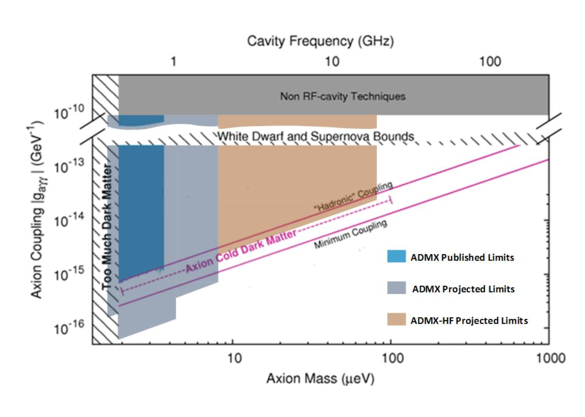
\includegraphics[width=150mm]{Figures/ADMX.png}
\caption{Long term projected limits of the ADMX and ADMX-HF experiments. \cite{ADMX}}
\label{fig:admx} 
\end{figure}

The previously cited limits are on axions that were formed in the cores of stars. These axions, if they existed, would not be able to fill the CDM role. Currently, the only experiment that would be sensitive to dark matter axions is the Axion Dark Matter Experiment (ADMX). This experiment aims to convert axions from the local dark halo into photons using a microwave resonant cavity permeated with a strong magnetic field. In this scenario, a DM axion would interact with a virtual photon from the magnetic field to convert into a real RF photon which can be detected. ADMX and it's sister experiment ADMX-HF are looking for axion dark matter in the mass range $2 \mu eV$ to $100 \mu eV$ and are expected to be able to probe most of the allowable axion CDM phase space\cite{axion_DM,ADMX}.





\subsection{WIMPs}
The other leading candidate for CDM is what is referred to as the Weakly Interacting Massive Particle, or WIMP. ``WIMP'' is a somewhat generic term for a massive particle that couples to standard model particles only through the weak nuclear force. This generic WIMP particle is usually denoted as $\chi$. Many extensions to the standard model, in particular supersymmetric models, include at least one flavor of WIMP. In the very early universe WIMPs will be in equilibrium with the primordial plasma. Just as with CMB photons and CNB neutrinos, once the temperature drops and the universe expands the number and temperature of WIMPs will fall out of equilibrium and the particles remaining will persist as a cosmic relic\cite{susyDM,wimp2}.

When the temperature of the universe is higher than the WIMP mass, $m_{\chi}$ (roughly 10  GeV to 1 TeV) both the WIMP number density, $n_{\chi}$, and temperature will be in thermal equilibrium. Once the temperature drops below the WIMP mass, the number density will fall out of equilibrium and will pick up a Boltzmann suppression factor of $e^{-m_{\chi}/T}$. Once the the scattering rate of cosmic WIMPs drops below expansion rate of the universe, $\chi$ particles will no longer be able to find each other to annihilate, and $n_{\chi}$ will freeze out, becoming the relic density that exists today\cite{wimp2}.

\begin{figure}[h!]
\centering
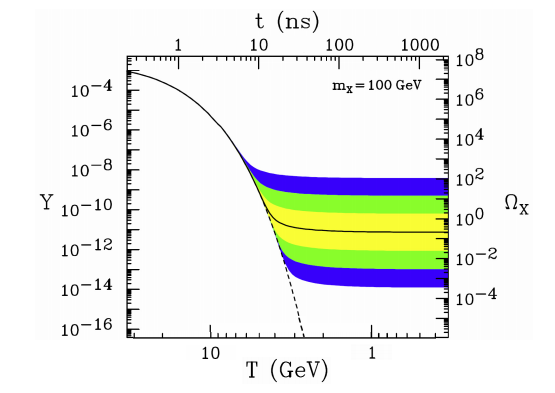
\includegraphics[width=150mm]{Figures/WIMP_relic_density.png}
\caption{WIMP number density in the early universe.The solid line corresponds to the cross section required to account for 100\% of CDM. The colored bands indicate variations by factors of 10, 100 and 1,000\cite{wimp2}.}
\label{fig:reldens} 
\end{figure}


This relic density is determined by the mass of $\chi$, as well as its self-annihilation cross section, $\sigma_{A}$, but is much more strongly dependent upon the cross section.\cite{susyDM,wimp2} If $\sigma_{A}$ is on the scale of the weak force, the density parameter for relic WIMPs will be on the order of what is required for $\Omega_{CDM}$. This is considered one of the most compelling reasons to consider WIMPs as CDM candidates, and has been referred to as the ``WIMP miracle''\cite{wimp1,wimp2, susyDM}.

The creation of the relic density is described by the Boltzmann equation:
\begin{equation}\label{eq:boltz}
\frac{dn_{\chi}}{dt} = -3Hn_{\chi}- \langle \sigma_{A}v \rangle (n_{\chi}^{2}-n_{eq}^{2}).
\end{equation}
In equation \ref{eq:boltz}, the first term on the right hand side is from the expansion of the universe, the $n_{\chi}^{2}$ term is from self annihilation, and the $n_{eq}^{2}$ is the creation of WIMPs from standard model particles.\cite{susyDM,wimp2} The value of $n_{eq}$ is what the number density of WIMPs would be in thermal equilibrium in a static universe. Equation \ref{eq:boltz} has no closed form solution and is solved numerically. There is, however, some insight that can be drawn from some rough analysis\cite{wimp1,wimp2}.

The equilibrium number density for non-relativistic dark matter is given by a simple Boltzmann distribution, $n_{\chi}=g_{\chi}\frac{m_{\chi} T}{2 \pi}e^{-m_{\chi}/T}$.\cite{wimp1} Freeze out will occur when the expansion rate of the universe, $H$, exceeds the annihilation rate of WIMPs, $\Gamma =  n_{\chi} \langle \sigma_{A}v \rangle $. In rough terms, the freeze out temperature can be defined as the temperature at  which $H$ and $\Gamma$ are equal.\cite{wimp1,wimp2}  In the early universe, it is appropriate to make the approximation $H \approx 1.66 g_{*}^{1/2}T^{2}$\cite{susyDM}. In this case the equation $H=\Gamma$ can be rewritten to give the WIMP density at freezeout:

\begin{equation}\label{eq}
n_{\chi,f}
\approx
g_{\chi}\frac{m_{\chi} T_{f}}{2 \pi}e^{-m_{\chi}/T_{f}} 
\approx 
\frac{1.66 g_{*}^{1/2}T_{f}^{2}}{\langle \sigma_{A}v \rangle }
\end{equation}

The ratio of $x_{f} \equiv m_{\chi}/T_{f}$ remains roughly constant between different WIMP models and has a value of about $1/20$. After freeze out, the ratio of $n_{\chi}$ to entropy density, $s$, is constant. In the early universe, $s \approx 0.4 g_{*}T^{3}$. Holding $(n_{\chi}/s)$ constant from freeze out to the present day yields the following expression for the current energy density, $n_{\chi,0}$:

\begin{equation}
n_{\chi,0} 
\approx
\frac{1.66 g_{*}^{1/2}T_{f}^{2}}{\langle \sigma_{A}v \rangle }
\cdot
\frac{s_{0}}{0.4 g_{*}T_{f}^{3}}
\end{equation} 

Taking the current entropy density to be $s_{0}=4000 cm^{-3}$ yields the following energy density for relic WIMPs:
\begin{equation}
\Omega_{\chi} h^{2}
\approx
\frac{3 \cdot 10^{-27} \ GeV \ cm^{3}}{\langle \sigma_{A}v \rangle}
\end{equation}

Plugging in a typical weak annihilation cross section of about $10^{-25} \ cm^{3} \ s^{-1}$ for $\langle \sigma_{A}v \rangle$ gives $\Omega_{\chi} h^{2} \approx 0.03 \ GeV \ s$ which is close enough to the expected value CDM, $\Omega_{CDM} h^{2} = 0.1188 \ GeV \ s$\cite{planck2015} to make WIMPs an extremely exciting candidate to explain much, if not all, of the non-baryonic dark matter in the universe\cite{susyDM,wimp2}.


\section{WIMP Direct Detection}
The relic density of WIMPs is determined by the cross-section for annihilation into standard model particles, a process which might be observed today by looking for high energy particles coming from high density regions of space such as galactic nuclei. The hypothetical interaction between WIMPs and standard model particles can also be run in two other directions. Production of WIMP dark matter from standard model particles can be searched for using modern particle colliders such as the LHC at CERN, and the scattering of relic dark matter can be probed for using large, low-background detectors. These three methods of detection are referred to as ``indirect detection'', ``production'', and ``direct detection'' respectively. Direct detection is of particular interest because it probes the existing relic dark matter background that is postulated by the $\Lambda$-CDM model.

\begin{figure}[h!]
\centering
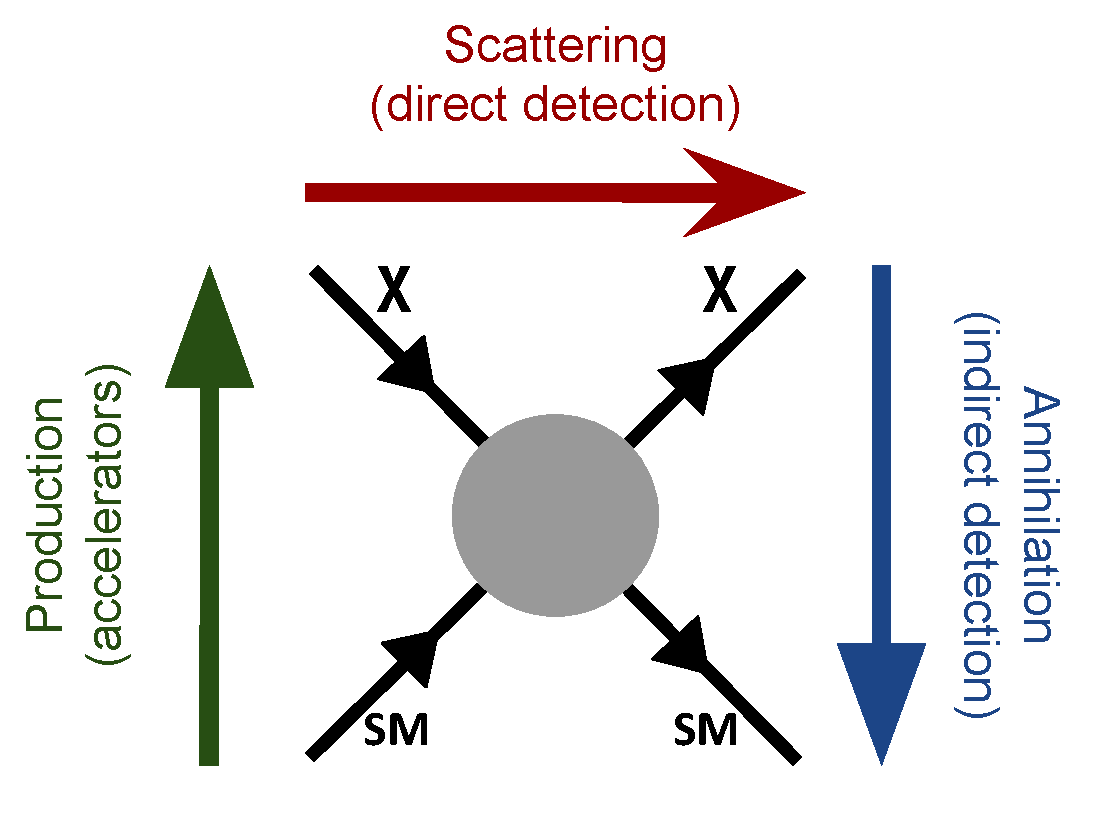
\includegraphics[width=150mm]{Figures/WIMP_interaction.pdf}
\caption{Cartoon of the WIMP-standard model interaction. The green, red, and blue arrows indicate in which direction time is being run for production, scattering, and annihilation, respectively.}
\label{fig:WIMP_SM} 
\end{figure}

\subsection{Recoil spectrum}
Direct detection experiments look for the of scattering a standard model nucleus off of a dark matter particle from the galactic halo. The expected rate and energy spectrum of such an interaction can be estimated assuming you know the local density and velocity of the WIMP halo. In this section, we also make the assumptions of spin independence of the interaction, along with the elasticity of the recoil, although models which violate these assumptions do exist.

The WIMP halo is expected to have only a small amount of bulk rotation; that is it is expected to be more akin to a gravitationally bound ideal gas than an accretion disk. The the expected velocity of a WIMP in such a halo would then be equal to $\vec{v_{\chi}}+\vec{v_E}$, with $\vec{v_{\chi}}$ being the expected velocity of a WIMP particle inside the halo, and $\vec{v_E}$ is the orbital velocity of the earth around the galactic center. The sun's orbital velocity is $v_s=230$ km/s.

The velocity of a WIMP in the lab frame will be dominated by $v_s$, which is highly non-relativistic. This being the case, collisions between WIMPs and the target nuclei of earth-bound detectors can be well modeled by classical elastic scattering. The recoil spectrum for this type of event is given by:
\begin{equation} \label{eq:recoilspec}
\frac{dR}{dE_{r}}=\frac{R_{0}}{E_{0}r}e^{-E_{r}/E_{0}r},
\end{equation}
where $R$ is the event rate per unit mass, $E_{r}$ is the recoil energy, $R_{0}$ is the total event rate, and $E_{0}$ is the most common incident WIMP energy. In equation \ref{eq:recoilspec}, $r$ is a kinematic factor given by $4M_{\chi}M_{N}/(M_{\chi}+M_{N})^2$, where $M_{\chi}$ is the mass of the dark matter particle, and $M_{N}$ is the mass of the target nucleus. 

From measurements of the galactic rotation curve, the local dark matter density is expected to be approximately 0.2-0.4 GeV cm$^{-3}$, although could be as high as 0.7 GeV cm$^{-3}$ given a nonuniform halo density profile\cite{weber}. 


\subsection{Cross Section}
The last ingredient needed to calculate the expected interaction rate in a give experiment is the scattering cross section. The WIMP-nucleus scattering cross section will have some dependence on the momentum transfer, $q$, and can be written\cite{dmintro}:
\begin{equation}
\sigma(q)=\sigma_0F(q),
\end{equation}
where $\sigma_0$ is the energy independent, 0-momentum limit of the cross section, and $F(q)$ is an energy dependent form factor. The 0-momentum cross section can be broken into a spin dependent (SD) part and a spin independent (SI) part\cite{wimp_nucleon,dmintro}:
\begin{equation}\label{eq:sisd_cs}
\begin{split}
\sigma_{0,SI}=& \frac{4\mu_A^2}{\pi}[Zf_p+(A-Z)f_n]^2 \\
\sigma_{0,SD}=& \frac{32G_F^2\mu_A^2(J+1)}{\pi J}[a_p\langle S_p \rangle + a_n\langle S_n \rangle ]^2
\end{split}
\end{equation} 
Here, $f_{p,n}$ and $a_{p,n}$ are the SI and SD coupling constants of WIMPs to protons and neutrons, $\mu_A$ is the reduced mass of the interaction, $Z$ is the atomic number, $A$ is the atomic mass, $J$ is the nuclear spin, and $\langle S_{p,n} \rangle$ is the average spin of protons or neutrons in the nucleus. It is typically assumed that $f_p \approx f_n$, so the SI cross section reduces to:
\begin{equation}\label{eq:sics}
\sigma_{0,SI}= \frac{4\mu_A^2}{\pi}f_n^2A^2. 
\end{equation} 

The $\mu_A^2A^2$ dependence in equation \ref{eq:sics} is a result of the non-relativistic nature of the interaction leading the incident WIMP to scatter coherently off of the nucleus as a whole as opposed to the individual nucleons. This is an important result because it indicates a large benefit to using heavy nuclei as experimental target media. For instance, a detector which uses xenon as its target medium (A$\approx$131) will be over 10 times more sensitive to a 100 GeV WIMP than an argon based detector (A$\approx$40) with the same mass of target material. 

Another important result is that the SD cross section does not have the same $\mu_A^2A^2$ dependence, and in many nuclei the nucleon spins cancel entirely leaving that isotope insensitive to WIMP interactions. In the case of xenon, the only isotopes that have non-zero spin and a non-negligible natural abundance are $^{131}$Xe (J=3/2) and $^{129}$Xe (J=1/2), which together make up just under half of the natural xenon abundance. Since for xenon has an even number of protons, $\langle S_p \rangle$ is very close to zero (-0.009 for $^{131}$Xe and 0.028 for $^{129}$Xe). The neutron part of the SD cross section in $^{129}$Xe and $^{131}$Xe is about 2,000 and 400 times that of a single-neutron, respectively. We can compare this to the SI cross section of xenon, which is $>5\times 10^7$ times larger than the single-nucleon cross section. This suppression of the SD cross section in comparison with the SI cross section has led to much less stringent limits on spin independent interactions than on spin dependent interactions as can be seen in the results from the LUX detector in figure \ref{fig:wimplimits}.
\begin{figure*}
        \centering
        \begin{subfigure}[b]{0.475\textwidth}
            \centering
            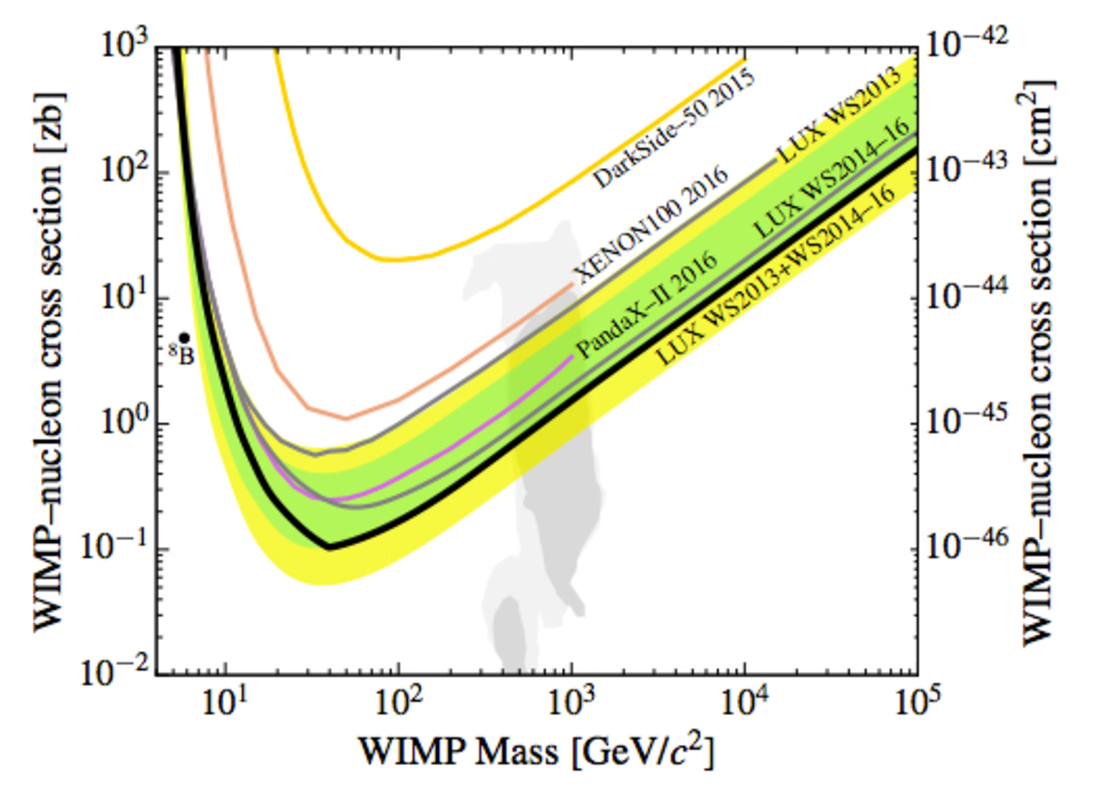
\includegraphics[width=\textwidth]{Figures/WIMP_nucleon.pdf}
            \caption{} 
            \label{fig:wimplimits_si}
        \end{subfigure}
        \hfill
        \vskip\baselineskip
        \begin{subfigure}[b]{0.475\textwidth}   
            \centering 
            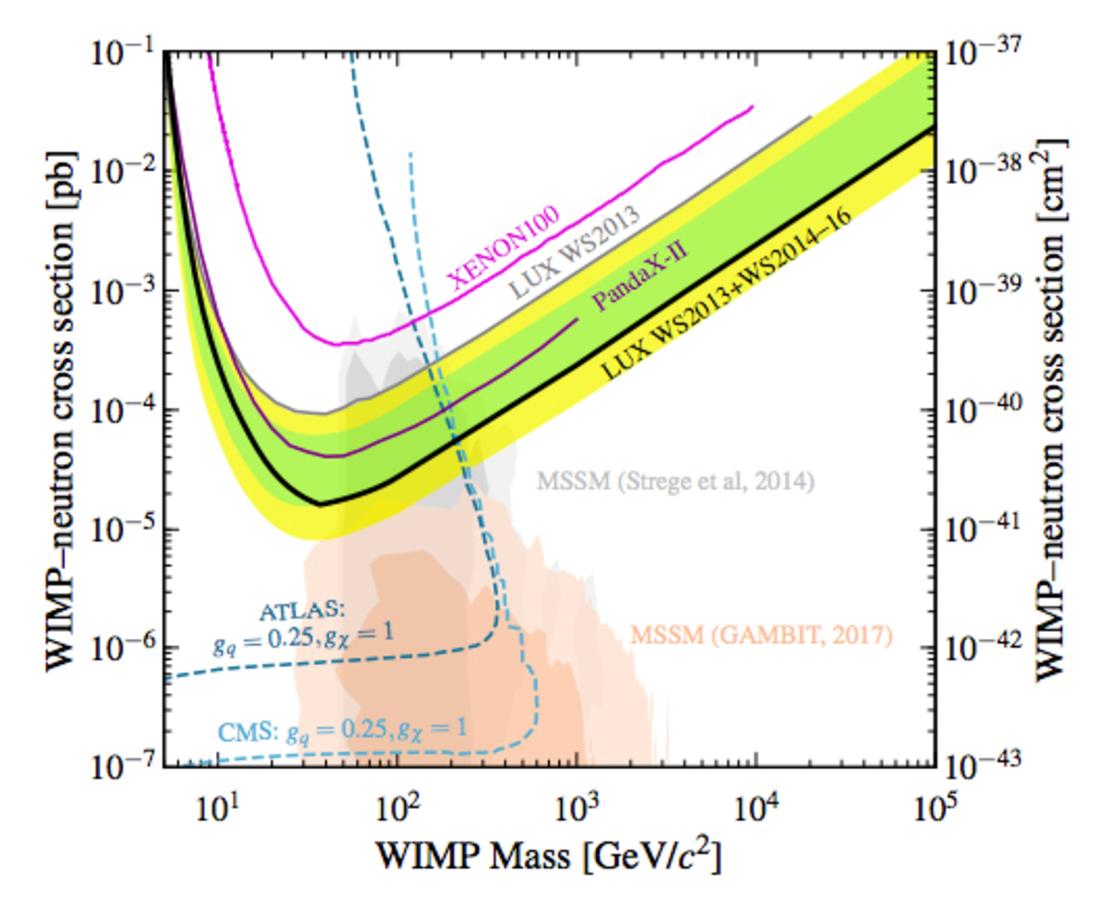
\includegraphics[width=\textwidth]{Figures/WIMP_neutron.pdf}
            \caption{}   
            \label{fig:wimplimits_sdn}
        \end{subfigure}
        \quad
        \begin{subfigure}[b]{0.475\textwidth}   
            \centering 
            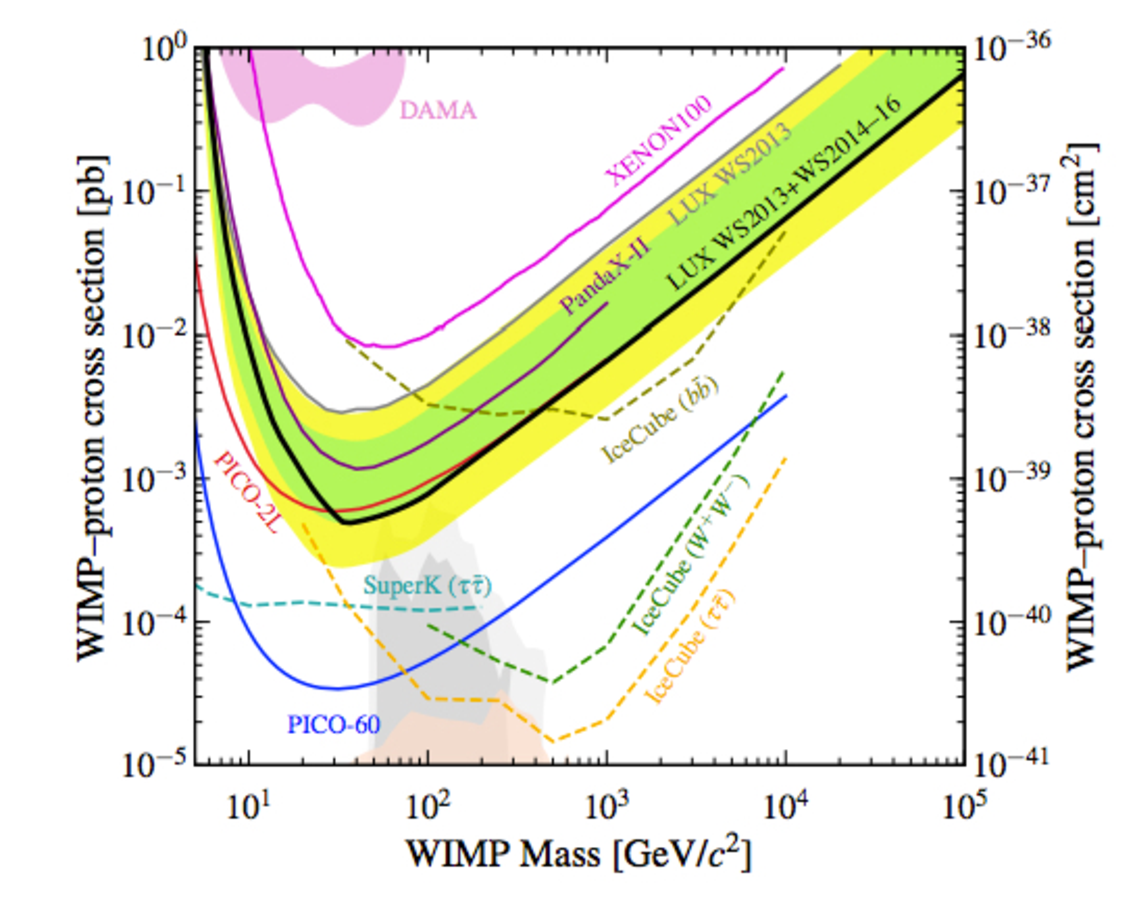
\includegraphics[width=\textwidth]{Figures/WIMP_proton.pdf}
            \caption{}
            \label{fig:wimplimits_sdp}
        \end{subfigure}
        \caption{Limits on the SI single-nucleon (a), SD single neutron (b), and SD single proton (c) cross sections. This limits were take from the LUX experiment's full exposure (332 days). The SI limit is roughly 5 orders of magnitude better than the SD neutron limit, which itself is about 2 orders of magnitude better than the SD proton limit. The solid black lines show the experimentally measured limits, and the green and yellow regions show the 1- and 2-$\sigma$ expectations. Figures were taken from \cite{lux_2017} and \cite{lux_sd}.}
        \label{fig:wimplimits}
    \end{figure*}


\section{Thesis Outline}
